\documentclass{article}

\usepackage{fullpage}
\usepackage{amsmath,amsfonts,amsthm,amssymb}

\usepackage{listings}
\usepackage{color}
\usepackage{graphicx}

\definecolor{dkgreen}{rgb}{0,0.6,0}
\definecolor{gray}{rgb}{0.5,0.5,0.5}
\definecolor{mauve}{rgb}{0.58,0,0.82}

\lstset{frame=tb,
  language=Python,
  aboveskip=3mm,
  belowskip=3mm,
  showstringspaces=false,
  columns=flexible,
  basicstyle={\small\ttfamily},
  numbers=none,
  numberstyle=\tiny\color{gray},
  keywordstyle=\color{blue},
  commentstyle=\color{dkgreen},
  stringstyle=\color{mauve},
  breaklines=true,
  breakatwhitespace=true,
  tabsize=3
}

\begin{document}
\title{CS 457, Data Structures and Algorithms I\\
Third Problem Set\\
Renju Radhakrishnan}
\maketitle
\begin{center}
\end{center}

\begin{enumerate}
\item \textbf{9.3-7}\\
Describe $O(n)$-time algorithm that, given a set $S$ of $n$ distinct numbers and a positive integer $k\leq n$, determines the $k$ numbers in $S$ that are closest to the median of $S$ \\ \\
{\textit{Answer}} \\
Given a set $S$ of $n$ distinct numbers, we select two values in between the $k$ value and compare the values in $S$ with those values. We can recursively call the algorithm until it finds the selected value. An easier algorithm is to find the median by using the median of median algorithm, then subtract that median from all values. Afterwards, take the absolute value of all the integers and find the smallest $kth$ value in the array. Thus, completing in $O(n)$ time.
\newpage
\item \textbf{9.2 Weighted Median}\\
For $n$ distinct elements $x_1, x_2, \dotso, x_n$ with positive weights $w_1, w_2, \dotso, w_n$ such that $$\sum_{x_i < x_k} w_i < 1/2$$ and $$\sum_{x_i > x_k} w_i < 1/2$$
For example, if the elements are 0.1, 0.35, 0.05, 0.1, 0.15, 0.05, 0.2 and each element equals its weight (that is, $w_i = x_i$ for $i$ = 1, 2, \dotso, 7), then the median is 0.1, but the weighted median is 0.2.
\subitem \textbf{a.} Argue that the median of $x_1, x_2, \dotso, x_n$ is the weighted median of the $x_i$ with weights $w_i$ = 1/$n$ for $i$ = 1, 2, \dotso, $n$. 

{\textit{Answer}}

Given $x_k$ as the median of $x_1, x_2, \dotso, x_n$ , by the definition of medians, $x_k$ is bigger than $(n + 1)/2 - 1$ elements as seen from $\sum_{x_i < x_k} w_i < 1/2$. On the other side of the median, $x_k$ is smaller than $(n - (n+1)/2$ elements, as shown from $\sum_{x_i > x_k} w_i < 1/2$. Thus, by definition of weighted medians $x_k$ is a weighted median.

\newpage
\subitem \textbf{b.} Show how to compute the weighted median of $n$ elements in $O(nlgn)$ worst-case time using sorting.

{\textit{Answer}}

In order to compute the weighted median of $n$ elements, we sort the list then add the weights of the medians until the median is found.

\begin{lstlisting}
def weighted-median(Set)
	int counter = 0;
	int weight = 0;
	while(weight + Set[i].weight < $1/2$) {
		weight = weight + Set[i].weight;
		counter++;
	}
	return weight;
	
\end{lstlisting}

\newpage

\subitem \textbf{c.} Show how to compute the weighted median in $\Theta(n)$ worst-case time using a linear-time median algorithm such as SELECT from Section 9.3

{\textit{Answer}}

We can compute the weighted median using a $\Theta(n)$ median algorithm through calculating the median then recursively searching on each half of the list to obtain the weighted median as shown below. 

\begin{lstlisting}
weighted-median(Set) {
	int median = set.getMedian();
	List list1, list2;	
	for(int i = 0; i < set.size(); i++) {
		if(Set[i] < median) {
			list1.append(Set[i]);
		} else {
			list2.append(Set[i]);
		}
	}
	if(list1.totalWeight > $1/2$)  {
		weighted-median(list1);
	} else {
		weighted-median(list2);
	}
}
\end{lstlisting}

\newpage
The \textbf{\textit{post-office location problem}} is defined as follows. We are given $n$ points $p_1, p_2, \dotso, p_n$ with associated weights $w_1, w_2, \dotso, w_n$. We wish to find a point $p$ (not necessarily one of the input points) that minimizes the sum $\sum_{i = 1}^{n} w_i d(p, p_i)$, where $d(a, b)$ is the distance between points $a$ and $b$.
\subitem \textbf{d.} Argue that the weighted median is a a best solution for the 1-dimensional post-office location problem, in which points are simply real numbers and the distance between points $a$ and $b$ is $d(a, b)$ = $|a-b|$.

{\textit{Answer}} 

We can show that the weighted median is the best solution for the 1-dimensional post-office location problem by choosing a $p$ to minimize the cost, rewriting it as a function of cost($p$) = $\sum_{i = 1}^{n} w_i d(p, p_i)$. We can rewrite the cost function as cost($p$) = $\sum_{p_i < p} w_i d( p - p_i)$ + $\sum_{i = 1}^{n} w_i d(p_i - p)$. Then we find the minimum through taking the derivative of cost with respect to p, thus $dc/dp$ = $(\sum_{p_i < p} w_i)$ - $(\sum_{p_i > p} w_i)$. Looking at the derivative, we can conclude that the function is greater than 0. 

\newpage

\subitem \textbf{e.} Find the best solution for the 2-dimensional post-office location problem, in which the points are (x, y) coordinate pairs and the distance between points $a = (x_1, y_1)$ and $b = (x_2, y_2)$ is the \textbf{\textit{Manhattan distance}} given by $d(a, b) = |x_1 - x_2| + |y_1 - y_2|$

This is the same problem as the 1-dimensional post-office location problem except for solving it separately for each dimension. Thus we can use the Manhattan distance to create a cost function where $p = (p_x, p_y)$ and cost($p$) = $(\sum_{i = 1}^{n} w_i |x_i - p_x|)$ + $(\sum_{i = 1}^{n} w_i |y_i - p_y|)$. We can follow the same steps for the 1-dimensional post-office location problem by taking the minimum value through derivation.

\newpage

\item \textbf{12-3 \textit{Average node depth in a randomly built binary search tree}}

In this problem, we prove that the average depth of a node in a randomly built binary search tree with $n$ nodes is $O(lgn)$. Although this result is weaker than that of Theorem 12.4, the technique we shall use reveals a surprising similarity between the building of a binary search tree and the execution of a RANDOMIZED-QUICKSORT from Section 7.3.
	
\hspace{10mm} We define the \textbf{total path length} $P(T)$ of a binary tree $T$ as the sum, over all nodes $x$ in $T$, of the depth of node $x$, which we denote by $d(x, T)$.

\subitem \textbf{a.} Argue that the average depth of a node in $T$ is $$1/n \sum_{x \in T} d(x, T) = 1/n P(T)$$ \hspace{11mm}Thus, we wish to show that the expected value of $P(T)$ is $O(nlgn)$. 

{\textit{Answer}} 

It is shown to be true as by definition the average depth of a node is the sum of all depths $1/n \sum_{x \in T} d(x, T)$ is divided by the total number of nodes $n$, thus proven.

\newpage

\subitem \textbf{b.} Let $T_L$ amd $T_R$ denote the left and right subtrees of tree $T$, respectively. Argue that if $T$ has $n$ nodes, then 

$P(T) = P(T_L) + P(T_R) + n - 1$. 

\textit{Answer}

Given a variable $x \in T_L$, this means that the length of the path for $x$ in $T$ is the path length for $x \in T_L$, in addition to the edge that connects the root. Thus, the same goes for $P(T_R)$. The height of the root of $T$ is 0 and the union of $P_L$ and $P_R$ is $n-1$, giving the initial equation $P(T) = P(T_L) + P(T_R) + n - 1$.

\newpage

\subitem \textbf{c.} Let $P(n)$ denote the average total path length of a randomly built binary search tree with $n$ nodes. Show that $$P(n) = 1/n   \sum_{i = 0}^{n-1} (P(i) + P(n - i - 1) + n - 1)$$

\textit{Answer}

If we start with the initial equation where $P(n, i)$ is the total path length of a binary search tree with total nodes $n$ with $i$ nodes in the left subtree , then using \textbf{b.} from the same problem, we can show that $P(n, i) = P(i) + P(n - i - 1) + n - 1$. We can then show the average of $P(n)$ as $P(n) = 1/n \sum_{k = 0}^{n - 1} P(n, i)$, which is simplified to $$P(n) = 1/n   \sum_{i = 0}^{n-1} (P(i) + P(n - i - 1) + n - 1)$$

\newpage

\subitem \textbf{d.} Show how to rewrite $P(n)$ as $$P(n) = 2/n \sum_{k= 1}^{n - 1} P(k) + \Theta(n)$$

\textit{Answer}

$$P(n) = 1/n \sum_{k = 0}^{n-1} (P(k) + P(n - k -1) + n - 1)$$
$$1/n\sum_{k = 0}^{n-1}(P(k) + P(n-k-1)) + 1/n\sum_{k=0}^{n-1}(n - 1)$$
$$P(n) = 1/n \sum_{k = 0}^{n-1} (P(k) + P(n - k -1)) + \Theta(n)$$

$$P(n) = 1/n \sum_{k = 0}^{n-1} (P(k) + P(n - k -1)) = P(0) + P(n - 1) \dotso P(1) + P(n-2)  \dotso P(n-1) + P(0)$$
$$P(n) = 2/n \sum_{k= 1}^{n - 1} P(k) + \Theta(n)$$

\newpage

\subitem \textbf{e.} Recalling the alternative analysis of the randomized version of quicksort given in Problem 7-3, conclude that $P(n) = O(nlgn)$.

$$P(n) = 2/n \sum_{k= 2}^{n - 1} P(k) + \Theta(n)$$
$$\sum_{k=2}^{n-1}klgk \leq 1/2n^2 lg(n) - 1/8n^2$$

which can be simplified to

$$\sum_{k=2}^{n-1}klgk = \sum_{k=2}^{n/2 -1}klgk + \sum_{k=n/2}^{n-1} klgk$$

afterwards, finding an upper bound

$$\sum{k=2}^{n-1} klg \leq lg n/2 \sum{k=2}^{n/2 -1} k +.lgn \sum{k=n/2}^{n-1}k$$

$$lgn \sum{k=2}^{n-1}k - \sum_{k=2}^{n/2-1}k \leq lgn((n-1)n)/2 - ((n/2 - 1)n/2)/2$$

$$\leq 1/2n^2lgn - 1/8n^2 where n\geq 2$$

Thus, through substitution

$$2c/n\sum{k=1}^{n-1} klgk.+ \Theta(n) \leq 2c/n(1/2 n^2lgn - 1/8n^2) + \Theta(n)$$
$$ \leq cnlgn$$

which holds true if $c/4n \geq \Theta(n)$

Thus $P(n) = O(nlgn)$


\newpage

At each recursive invocation of quicksort, we choose a random pivot element to partition the set of elements being sorted. Each node of a binary search tree partitions the set of elements that fall into the subtree rooted at that node.

\subitem \textbf{f.} Describe an implementation of quicksort in which the comparisons to sort a set of elements are exactly the same as the comparisons to insert the elements into a binary search tree. (The order in which comparisons are made may differ, but the same comparisons must occur.) 

\textit{Answer}

With quicksort, we know that the elements in the left and right partitions are never compared along with all elements after the chosen pivot are compared. Additionally, we know that binary search tree insertion results in a comparison to the root for all nodes inserted after it. The elements inserted into the respective subtrees are never compared to the opposite side either, e.g. the left subtree does not compare itself against the right subtree. Thus, a quicksort implementation that chooses the pivot in the same order as elements inserted into a binary tree will function the same way.

\newpage

\item \textbf{12.2-8}

Prove that no matter what node we start at in a height-$h$ binary search tree, $k$ successive calls to TREE-SUCCESSOR take $O(k + h)$ time. 

\textit{Answer}

We can prove this by initially starting with k successive calls of TREE-SUCCESSOR starting from element $x$, there are are most $h$ elements smaller than $x$ visited, and at most $h$ elements greater than $x+k$ visited. Thus, elements > $x+k$ are visited only when going down the tree. 

Elements between $x$ and $x + k$ are visited at most twice, once up and once down the tree. Given two nodes where $b$ is the left child of $a$, then before visiting $a$, the all elements greater than $x$ are visited in the left subtree. After those nodes are visited, then $a$ is visited. Given if $b$ is the right child, then after $a$ is visited, TREE-SUCCESSOR gets the minimum element in $b$'s right subtree. The area in the tree is not traversed again. Thus, giving $O(h + k)$.
\newpage. 

\item \textbf{13-3 AVL trees}

An \textbf{AVL tree} is a binary search tree that is \textbf{height balanced}: for each node $x$, the heights of the left and right subtrees of $x$ differ by at most 1. To implement an AVL tree, we maintain an extra attribute in each node: $x.h$ is the height of node $x$. As for any other binary search tree $T$, we assume that $T.root$ points to the root node. 

\subitem \textbf{a.} Prove that an AVL tree with $n$ nodes has height $O(lgn)$. ($Hint$: Prove that an AVL tree of height $h$ has at least $F_h$ nodes, where $F_h$ is the $h$th Fibonacci number.) 

\textit{Answer}

Given an AVL tree, we can let the $T(h)$ be the minimum number of nodes in a tree with a tree of height $h$. We can prove that an AVL tree with $n$ nodes has height $O(lgn)$ through induction. For the base case, $T(1) \geq T(0) \geq 1$, thus $T(1) \geq F_1$ and $T(0) \geq F_0$.  

$T(h') \geq F_h'$ for all $h' < h$

The AVL tree root height $h$ has two child nodes with heights $h-1$ and $h-2$. Thus the min number of nodes is shown by $T(h-1)$ and $T(h-2)$. Through induction, $T(h) \geq F_x + F_y = F_h$ where $ x = h - 1$ and $y = h-2$. This concludes that $h=O(lgn)$

\newpage

\subitem \textbf{b.} To insert into an AVL tree, we first place a node into the appropriate place in binary search tree order. Afterward, the tree might no longer be height balanced. Specifically, the heights of the left and right children of some node might differ by 2. Describe a procedure BALANCE($x$), which takes a subtree rooted at $x$ whose left and right children are height balanced and have heights that differ by at most 2, i.e, $|x.right.h - x.left.h| \leq 2$ , and alters the subtree rooted at $x$ to be height balanced. ($Hint$: Use rotations.)

\textit{Answer}

There are two situations that result in the AVL tree being unbalanced after insertion. The tree is no longer height balanced due to one side of the tree having a larger height. To check for a height-balanced AVL tree, we start by checking if the height are less than or equal to 1, if they are, then it is balanced. Otherwise, if the left height is greater than the right height, then left-rotate the left side. If the right height is greater, then we right rotate and continue to do so until the tree is balanced.

\newpage

\subitem \textbf{c.} Using part (b), describe a recursive procedure AVL-INSERT(x, z) that takes a node $x$ within an AVL tree and a newly created node $z$. (whose key has already been filled in), and adds $z$ to the subtree rooted at $x$, maintaining the property that $x$ is the root of an AVL tree. As in TREE-INSERT from Section 12.3, assume that $z.key$ has already been filled in and that $z.left = NIL$ and $z.right = NIL$; also assume that $z.h = 0$. Thus, to insert the node $z$ into the AVL tree $T$, we call AVL-INSERT(T.root, z).

\textit{Answer} 

We can create a resursive insert function that takes in two parameters $x$ and $z$. We first create a termination statement by checking if $x$ is $NIL$ then setting $height[z] = 0$ and returning $z$. If the base case isn't met, then check if the key at position $z$ is less than or equal to the key at $x$. if the statement is true, then call insert with the parameters $(left[x], z)$ and set that to a variable $a$. Afterwards set $left[x]$ to a, the parent node at $y$ to $x$ and the height $x$ to height $y$ + 1. If the key at $z$ is greater than the key at $x$, then call insert with $(right[x], z)$ and set $right[x]$ to a and follow the same procedures as the previous part. Finally, call the balance method from part (b) on $x$ then return it. This will maintain the balance of the tree while inserting a node. 

\newpage

\subitem \textbf{d.} Show that AVL-INSERT, run on an $n$-node AVL tree, takes $O(lgn)$ time and performs $O(1)$ rotations.

\textit{Answer}

Since we know that the height of an AVL tree is $O(lgn)$, thus the insertion and update on the tree height will take $O(lgn)$. The balance function decreases the height of the tree by 1, thus it wont affect the rest of the tree. This means that the insert takes at worst case $O(lgn)$ with a constant rotation of $O(1)$. 

\newpage

\item (15 pts) You are given a red-black tree $T$ with 15 internal nodes (nodes that hold key values) 
that form a \emph{full} binary tree of height 3 (i.e., a full binary tree of height 4 if you include 
the NIL leaves). Can you assign colors to the nodes so that a call to \textsc{RB-Insert}($T,z$) for
\emph{any} new key value $z.key$ will cause \textsc{RB-Insert-Fixup}($T,z$) to change the color of the 
root to red before switching it back to black? The initial assignment of colors needs to obey the 
red-black properties. If such a color assignment exists, then provide a sequence of 15 numbers whose 
insertion (in that order) would lead to such a tree, along with a figure of the resulting tree. If not, 
then explain why such an assignment cannot exist, using the fact that the tree needs to satisfy the 
red-black properties.

$1,2,3,4,5,6,7,8,9,0,1,3,2,4,5$

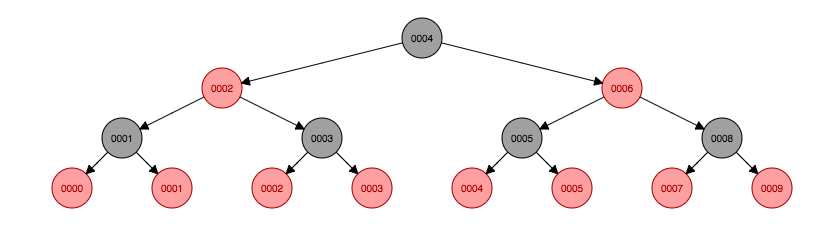
\includegraphics[scale=0.6]{rbt}

Any value inserted into the tree at this point will result in the root turning red then back to black as the leaves are all red along with the roots two children. 

\newpage

\item (12 pts) Provide an algorithm that, given a graph $G=(V,E)$ as input, decides whether $G$ is
bipartite. Also, provide a tight bound regarding the worst-case running time of the algorithm (show
how you got this bound), and explain why your algorithm is correct.

\textit{Answer}

We can use $BFS$ to check whether a graph $G$ is bipartite or not. First, we assign a red color to the initial vertex. Afterwards, color its neighbors blue. Then color the neighbor's neighbors with a red color. While coloring the vertexes if there is a neighbor that is colored the same color as the current vertex, then the graph is considered to not be a bipartite graph. Since we're using breadth first search to traverse the graph by coloring each node, our worst case run time complexity is $O(V + E)$. Since the algorithm will always traverse the entire graph to check whether it is bipartite, the runtime is always $O(V + E)$, thus giving a tight bound of $\theta (V + E)$. The algorithm itself is correct as a bipartite graph is one that has vertices that are divided into two sets. Coloring each consecutive set red then blue will result in the graph being either bipartite or the algorithm running into a neighbor colored with the same color as the current vertex, thus not being bipartite. Thus, the algorithm holds. 

\end{enumerate}
\end{document}